\chapter{Introduction}

\begin{quote}
    "What does it mean to see?" The plain man's answer (and Aristotele's, too) would be, to know what is where by looking. In other words, vision is the process of discovering from images what is present in the world and where it is.
\end{quote}
\begin{flushright}
    — David Marr
\end{flushright}

\begin{definitionblock}[Computer Vision]
    Computer vision is concerned with the automatic extraction, analysis and understanding of useful information from a single image or a sequence of images. It involves the development of a theoretical and algorithmic basis to achieve automatic visual understanding.
\end{definitionblock}

\begin{figure}[H]
    \centering
    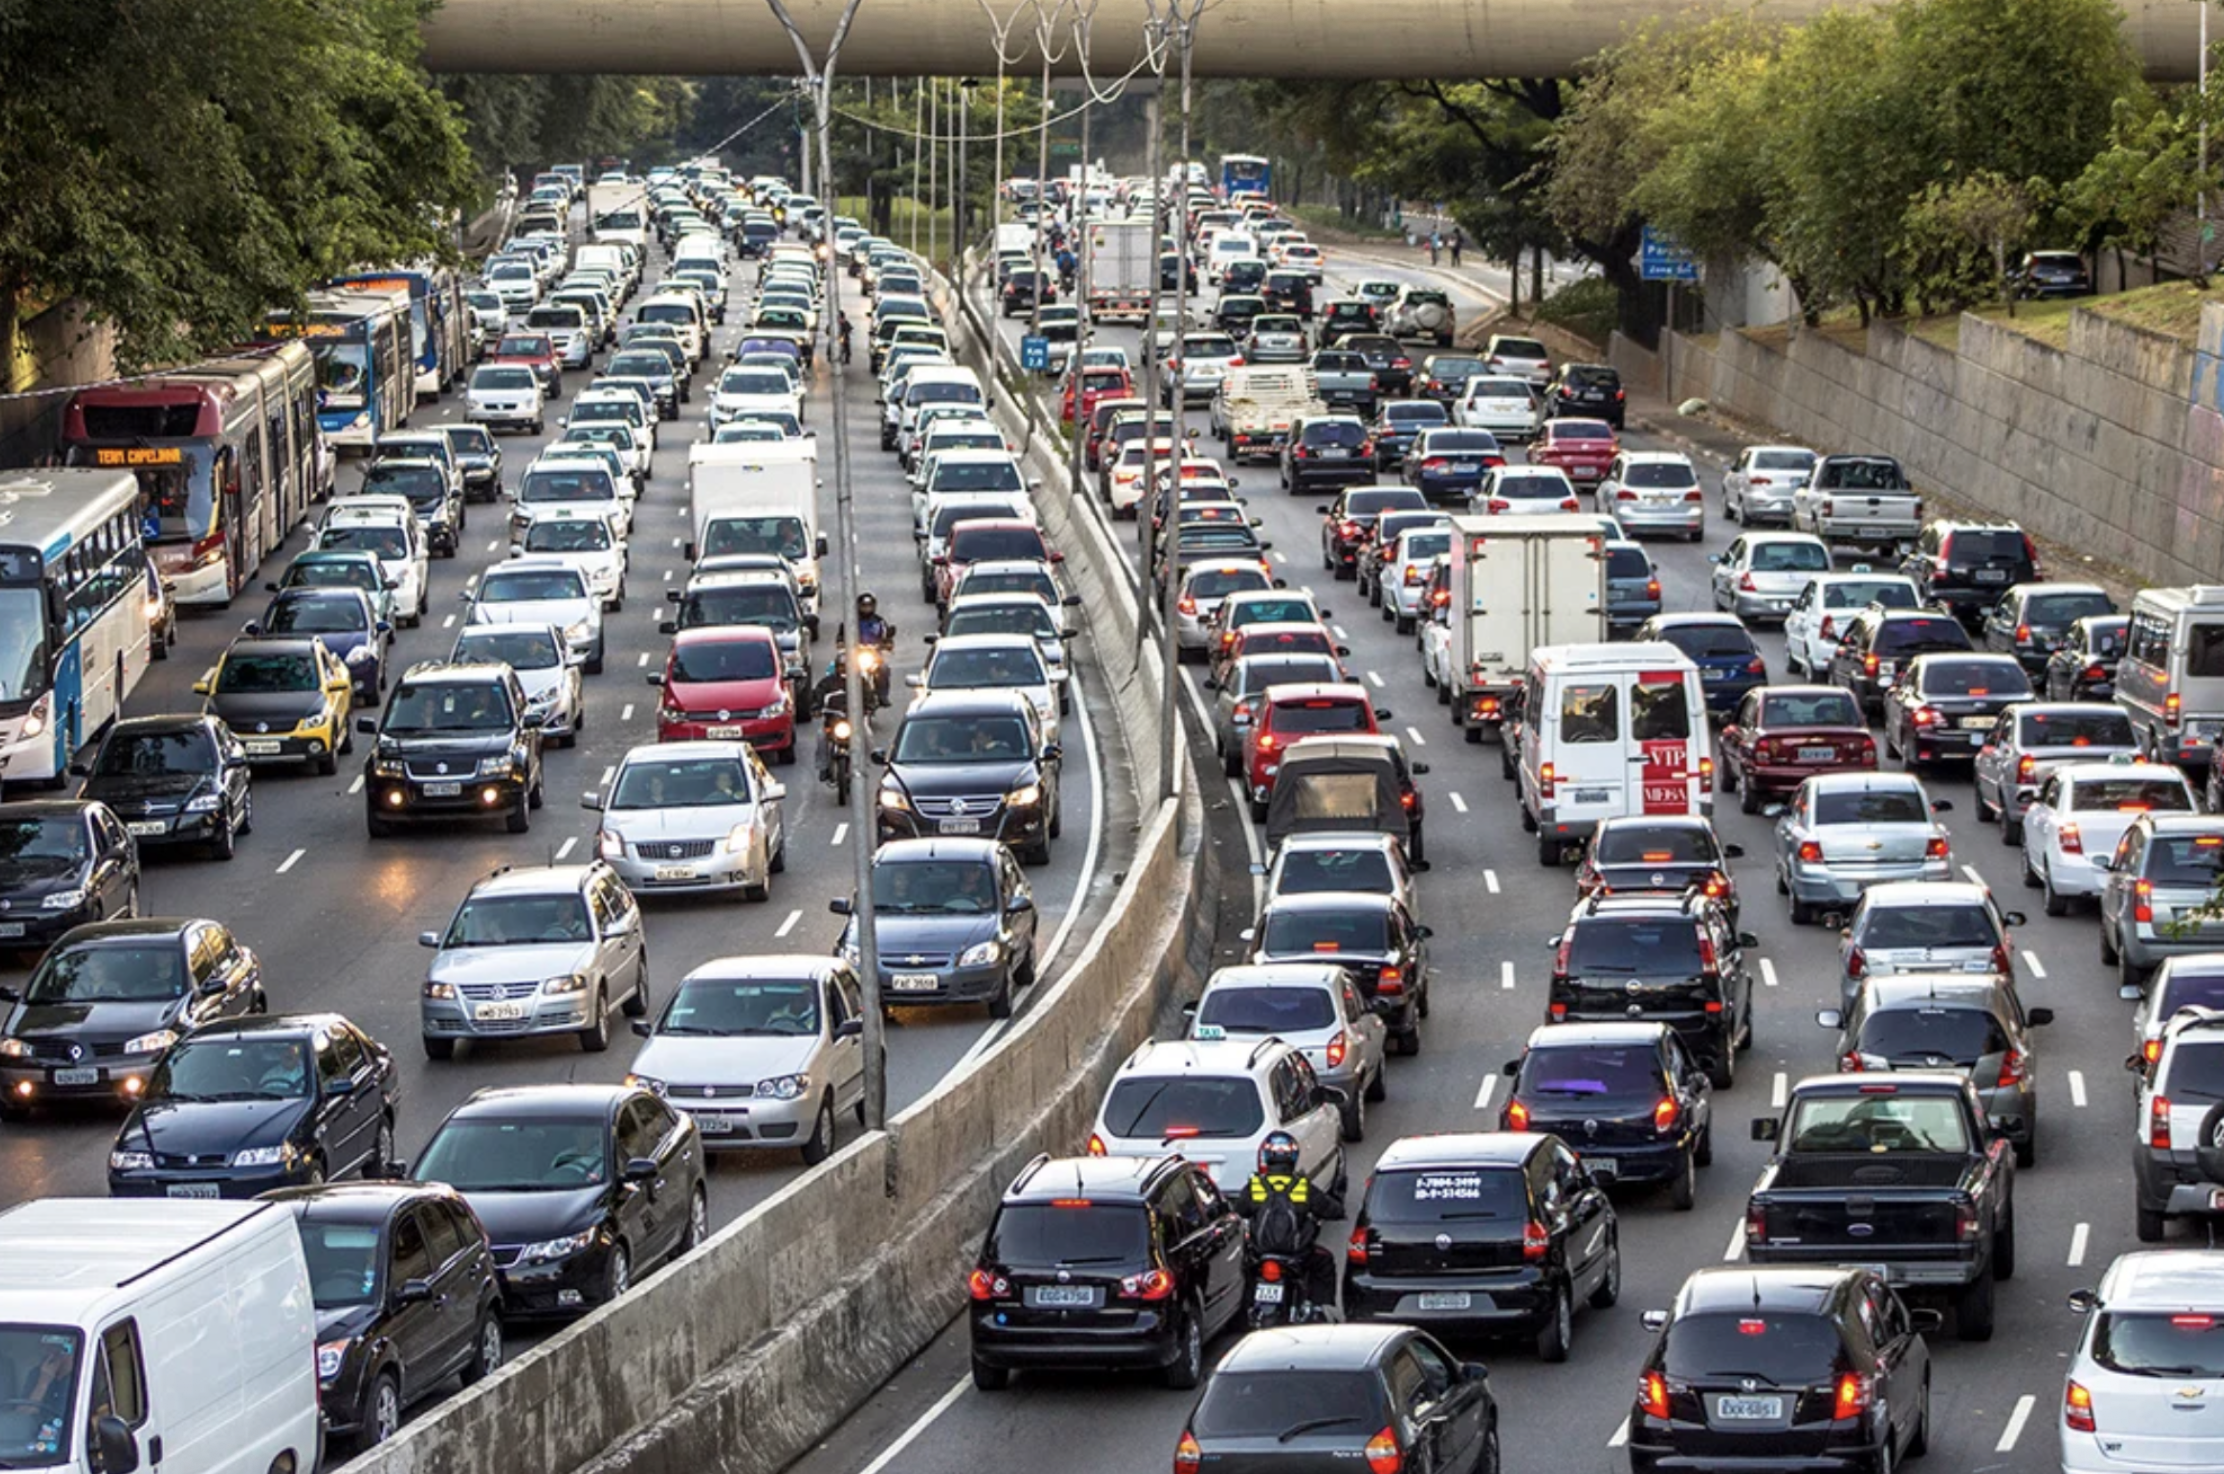
\includegraphics[width=0.6\textwidth]{assets/ch1/1.png}
    \caption{What is Computer Vision related to?}
    \label{fig:1}
\end{figure}

What can we extract from an image?
\begin{itemize}
    \item \textbf{Semantic Information} $\rightarrow$ "what"
    \item \textbf{Metric 3D Information} $\rightarrow$ "where"
\end{itemize}

\newpage
\paragraph{What} is difficult to define, since images are sensed and therefore represented in computers as arrays of numbers. Such low-level representation is far from \textbf{semantics}. One of the goals of CV is to bridge the gap between pixels and "meaning".

Examples include 3D surface reconstruction using either calibrated or uncalibrated images (with or without a model of the camera), dense matching of images, motion analysis, and tracking of objects in image sequences.

What is correct depends on the specific tasks, since a major problem in computer vision is the ambiguity of the visual data. For example, a single 2D image can be generated by an infinite number of 3D scenes. Therefore, additional constraints are needed to solve the problem. There are different levels of interpretation in this field. 

\paragraph{Where} is difficult as well; we go from 3D (world) to 2D (image) usually, but in understanding what is in the image we infer from 2D to 3D and in this process we loose information. 
\begin{itemize}
    \item The forward problem is well-posed (3D $\rightarrow$ 2D);
    \item The inverse problem is ill-posed (2D $\rightarrow$ 3D).
\end{itemize}

\begin{figure}[H]
    \centering
    \includegraphics[width=\textwidth]{assets/ch1/2.png}
    \caption{The forward and inverse problems.}
    \label{fig:2}
\end{figure}

Why people usually underestimates the difficulties of vision? Well, it is because we are pretty good at this task. There are special mechanisms in human vision that let us process low-level features such as size (length) and intensity in a non-trivial way.
\begin{itemize}
    \item Human vision may inspire, but most CV deals with finding effective ways for solving specific problems;
    \item there is no "the" CV algorithm, but instead a \textbf{collection of algorithms/approaches} for tackling \textbf{specific problems} in \textbf{restricted domains}.
\end{itemize}

Two classes of problems come from the "where" and "what" tasks:
\begin{enumerate}
    \item \textbf{Reconstruction} $\rightarrow$ recovering the 3D structure or a scene, given a sufficient amount of images of the object/scene;
    \item \textbf{Recognition} $\rightarrow$ here we can find object detection (find all the regions in an image where a specific kind of object is likely to occur), instance recognition (recognize a known specific object potentially being viewed from a novel viewpoint) or category-level recognition (categorize images as belonging to a general class such as "cat" or "bicycle", among many possible classes).
\end{enumerate}

\section*{Two noticeable achievements in CV}

\begin{itemize}
    \item \textbf{Uncalibrated reconstruction (Agarwal et al., 2011)}
    
    \begin{minipage}{0.48\textwidth}
        \begin{itemize}
            \item 496 processors
            \item 1984 GB of total memory 
            \item 62 TB of disk space
            \item 460000 Flickr pictures of Rome, Venice and Dubrovnik
            \item $\approx$ 100 hrs of computation
            \item Output: detailed 3D geometry and colors of monuments in Rome, Venice and Dubrovnik
        \end{itemize}
    \end{minipage}
    \begin{minipage}{0.48\textwidth}
        \centering
        \includegraphics[width=0.8\textwidth]{assets/ch1/3.png}
    \end{minipage}

    \item \textbf{Image categorization (Krizhevsky et al., 2012)}
\end{itemize}

\begin{observationblock}[Object's position in space]ù
    To specify the position of an object in space we need 6 parameters:
    \begin{itemize}
        \item 3 for translation (x, y, z);
        \item 3 for rotation (roll, pitch, yaw).
    \end{itemize}
\end{observationblock}

\section*{Applications}

\begin{figure}[H]
    \centering
    \includegraphics[width=0.8\textwidth]{assets/ch1/4.png}
    \caption{Some applications of Computer Vision.}
    \label{fig:3}
\end{figure}

\section*{About notation}

In most of the cases:
\begin{itemize}
    \item vectors are denoted by lowercase italic (e.g., $v$);
    \item scalars are denoted by mixed case italic (e.g., $\gamma$, $A$);
    \item matrices are denoted by uppercase italic (e.g., $M$);
    \item vectors operate as column vectors, i.e., they post-multiply matrices (e.g., $Mv$);
    \item transposition is denoted by $^T$;
    \item $v_1$ denotes a vector $v_1$ or the first component of vector $v$, or the first column of matrix $V$;
    \item $v_1^T$ denotes the first row of matrix $V$ or the transpose of vector $v_1$;
    \item $P \succ 0$ means that the matrix $P$ is positive definite;
    \item $P \succeq 0$ means that the matrix $P$ is positive semi-definite;
    \item $\nabla f$ denotes the gradient of function $f$ and is, by convention, a column vector;
\end{itemize}
